%------------------------- ADDITIONAL MATERIAL -------------------------%
\section{Additional Material} \label{app:additional_material}

%------------------------- MASS MOMENT OF INERTIA -------------------------%
\subsection{Mass Moment of Inertia of Square Tube} \label{app:mass_moment_of_inertia}

All moments of inertia are calculated assuming constant density $\rho$.
The thigh linkage is modeled as a cylindrical or square tube (subject to change).
In the case of a cylindrical tube, the moment of inertia around an axis as shown in Figure \ref{fig:inertia_cylinder} takes either of the following forms \cite{wikipedia_list_2019}

\begin{gather}
    I = \frac{\pi\rho h}{12} (3 (r_2^4 - r_1^4) + h^2 (r_2^2 - r_1^2))
    \\
    I = \frac{1}{12} m (3 (r_2^2 + r_1^2) + 4h^2)
\end{gather}

\begin{figure} [H]
    \centering
    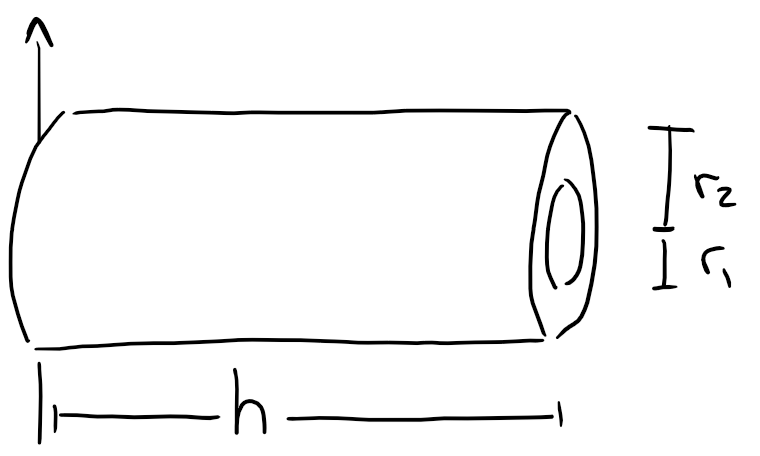
\includegraphics{4_ComponentProperties/img/inertia_cylinder.png}
    \caption{Mass Moment of Inertia of Cylindrical Tube}
    \label{fig:inertia_cylinder}
\end{figure}

In the case of a square tube, the general formula is not readily available  and must be derived.
The derivation follows the variables outlined in Figure \ref{fig:inertia_square_tube}.

\begin{figure}
    \centering
    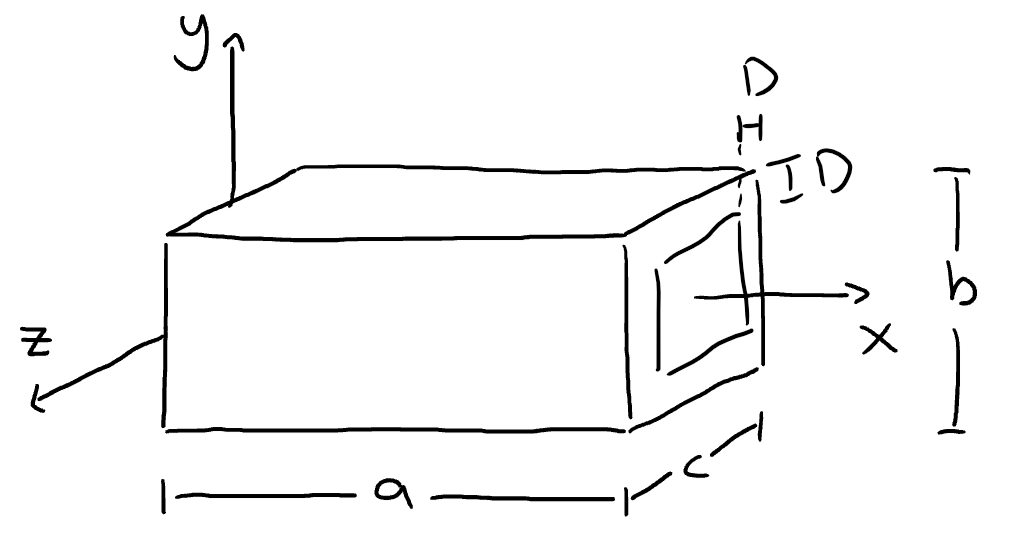
\includegraphics{4_ComponentProperties/img/inertia_square_tube.png}
    \caption{Mass Moment of Inertia of Square Tube}
    \label{fig:inertia_square_tube}
\end{figure}

%---------------------------------------

\begin{figure}[H]
    \centering
    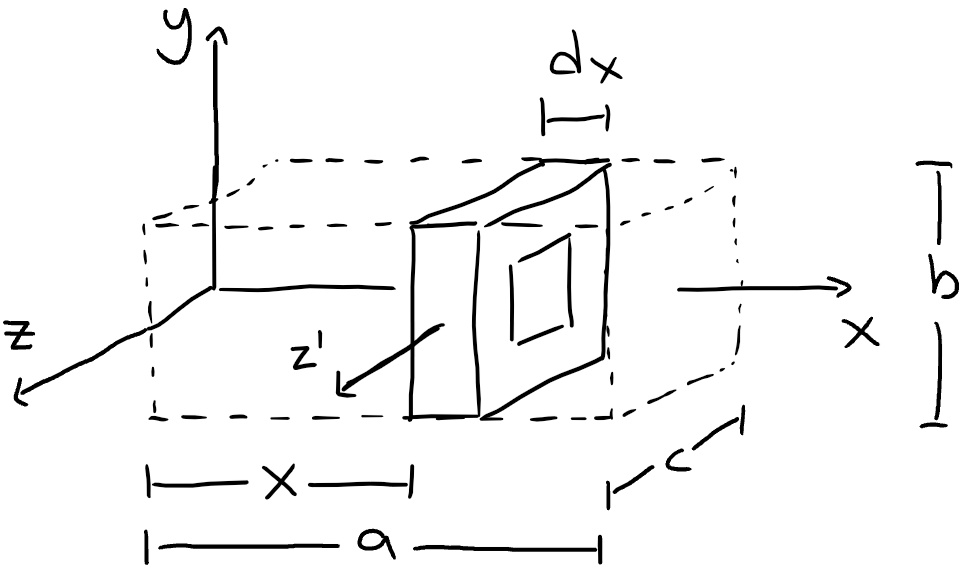
\includegraphics{7_Appendices/img/inertia_square_tube_slab.png}
    \caption{Mass Moment of Inertia of Square Tube - Slab view}
    \label{fig:inertia_slab}
\end{figure}

To compute the mass moment of inertia of a square tube, we must first determine the differential mass of a slab shown in Figure \ref{fig:inertia_slab}

\begin{equation}
    dm = \rho(bc - \big[(c-2D)(b-2D)\big])dx = \rho\big(2(b+c)D-4D^2\big)dx
\end{equation}

We then find the differential mass moment of inertia relative to the local axis $z'$ \cite{ferdinand_mass_2016}

\begin{equation}
    dI_{z'} = \rho dx I_{z',area} = \rho dx \frac{cb^3 - (c-2D)(b-2D)^3}{12}
\end{equation}

where $I_{z',area}$ is the area moment of inertia (or second moment of inertia) of the slab face \cite{engineers_edge_area_nodate}.
The differential mass moment of inertia relative to the global $z$ axis can thus be found using the parallel axis theorem \cite{ferdinand_mass_2016}

\begin{gather}
    dI_z = dI_{z'} + x^2 dm
    \\
    dI_z = \rho dx I_{z',area} + x^2 dm
    \\
    dI_z = \rho I_{z',area} dx  + x^2 \rho\big[2(b+c)D-4D^2\big]dx
    \\
    dI_z = \rho \big( I_{z',area} + \big[2(b+c)D-4D^2\big] x^2 \big) dx
\end{gather}

Finally, the expression is integrated with respect to $a$, giving the mass moment of inertia of the tube

\begin{gather}
    I_z = \rho \int_0^a I_{z',area} + \big[2(b+c)D-4D^2\big] x^2 dx
    \\
    I_z = \rho a \big[ I_{z',area} + \frac{1}{3}\big(2(b+c)D-4D^2\big) a^2 \big]
    \\
    I_z = \rho a \big( \frac{c b^3 - (c-2D)(b-2D)^3}{12} + \frac{1}{3}\big(2(b+c)D-4D^2\big) a^2 \big)
\end{gather}

In the case of a square tube, $b = c$, and so the expression becomes

\begin{equation}
    I_z = \rho a \big( \frac{b^4 - (b-2D)^4}{12}  + \frac{1}{3}\big(4b D-4D^2\big) a^2\big)
\end{equation}

The mass moment of inertia of composite bodies (composed of multiple bodies) can be calculated as the sum of all mass moments of inertia of the composite body, relative to the axis around which the inertia is being measured.

\begin{equation}
    I_{composite body} = \sum_i I_i
\end{equation}

The moment of inertia around the hip, for example, would be:

\begin{equation}
    I_{hip} = I_{thigh} + I_{knee} + I_{tibia} + I_{foot}
\end{equation}

Alternatively, a simple and conservative approximation of the linkage moments of inertia can be found using the inertia matrix in Subsection \ref{subsec:dynamic_equation}.



%------------------------- DYNAMIC EQUATION -------------------------%
\subsection{Generalized Equation of Motion} \label{app:dynamic_equation}

The following derivation allows for a single vector equation that provides the resulting joint torques for a given configuration and acceleration.
A side view of the leg $i$ is shown in Figure \ref{fig:dynamic_leg_app}.
From now on, the letter $i$ shall be dropped from all notation to speed up equation writing; all variables are still with respect to leg $i$.

\begin{figure}[H]
    \centering
    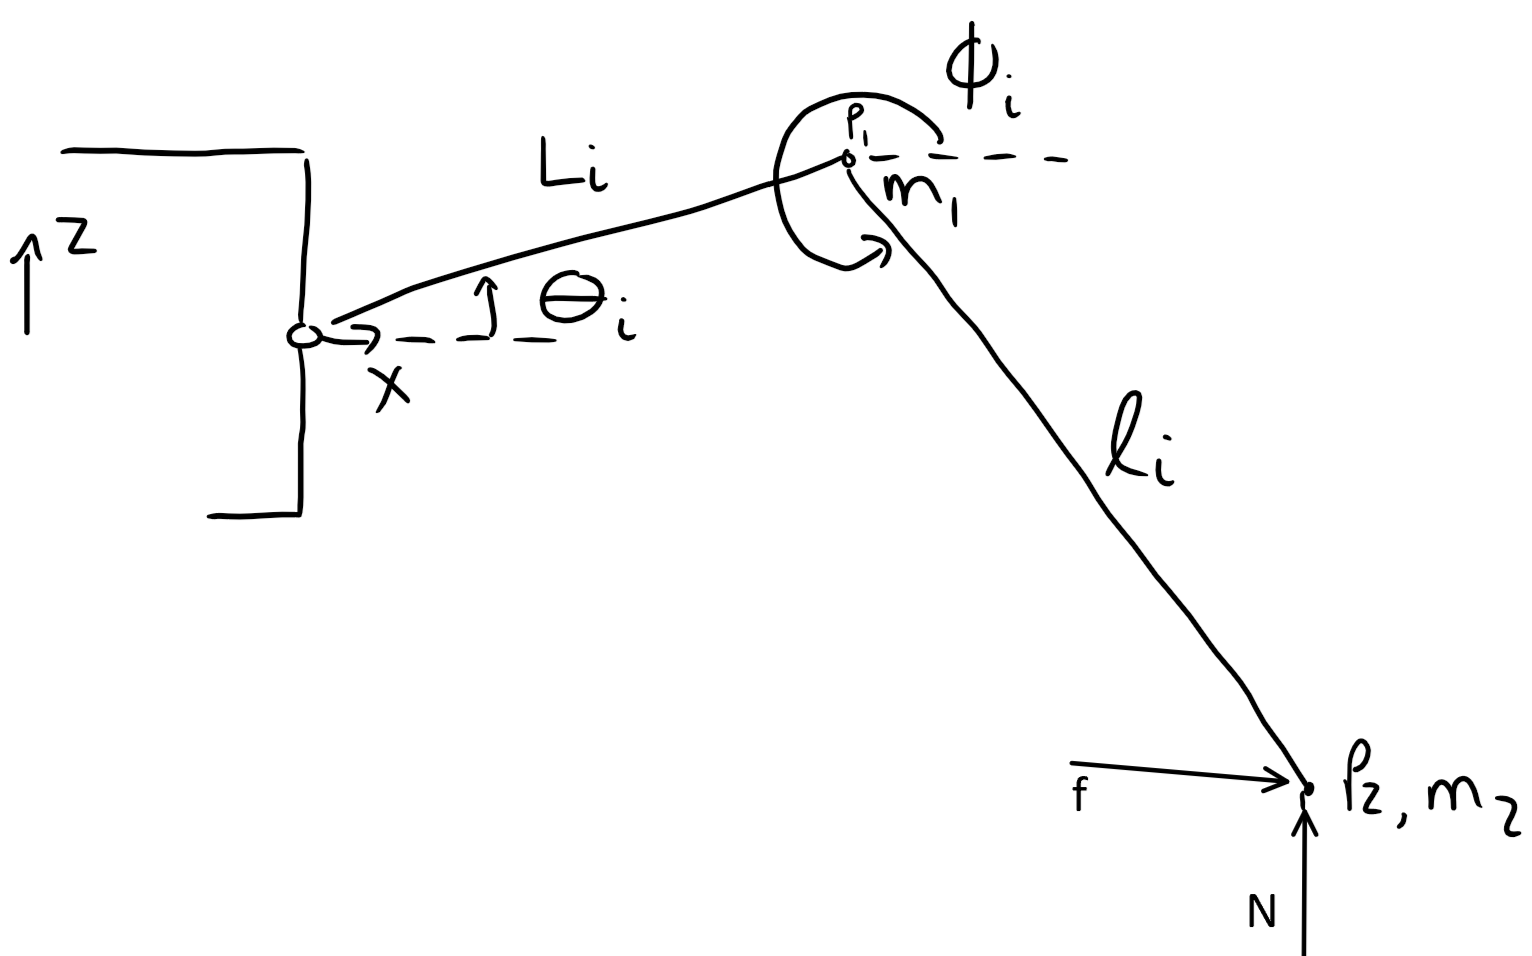
\includegraphics[width=\textwidth]{5_KinematicAndForces/img/dynamic_leg.png}
    \caption{Side View of Leg $i$}
    \label{fig:dynamic_leg_app}
\end{figure}

The positions of points $P_1$ and $P_2$ in $x$ and $z$ are given in vector form

\begin{gather}
    P_1 = \begin{bmatrix} L \cos \theta \\ L \sin \theta \end{bmatrix}
    \\
    P_2 = \begin{bmatrix} L \cos \theta + \ell \cos \phi \\ L \sin \theta + \ell \cos \phi \end{bmatrix}
\end{gather}

After deriving once

\begin{gather}
    P_1 = \begin{bmatrix} 
        -L\dot{\theta}\sin\theta \\
        L\dot{\theta}\cos\theta
        \end{bmatrix}
    \\
    P_2 = \begin{bmatrix}
        -L\dot{\theta}\sin\theta - \ell\dot{\phi}\sin\phi\\
        L\dot{\theta}\cos\theta + \ell\dot{\phi}\cos\phi
        \end{bmatrix}
\end{gather}

In explicit matrix form:

\begin{gather}
    P_1: \begin{bmatrix} \dot{x} \\ \dot{z} \end{bmatrix} = \begin{bmatrix}
        -L\sin\theta & 0 \\
        L\cos\theta & 0
        \end{bmatrix} \begin{bmatrix} \dot{\theta} \\ \dot{\phi} \end{bmatrix} \label{eq:jacobian_1}
    \\
    P_2: \begin{bmatrix} \dot{x} \\ \dot{z} \end{bmatrix} = \begin{bmatrix}
        -L\sin\theta & -\ell\sin\phi \\
        L\cos\theta & \ell\cos\phi
        \end{bmatrix} \begin{bmatrix} \dot{\theta} \\ \dot{\phi} \end{bmatrix} \label{eq:jacobian_2}
\end{gather}

Where the $4 \times 4$ matrices are Jacobians $J_1$ and $J_2$.
The inertia matrix is given by

\begin{equation} \label{eq:inertia_matrix_general}
    M = m_1 J_1^T J_1 + m_2 J_2^T J_2 = [kg][m][m] + [kg][m][m]
\end{equation}

This matrix approximates the inertial component of the necessary motor torques conservatively by approximating the entire mass of the linkages at the joints.
After substituting in \ref{eq:jacobian_1} and \ref{eq:jacobian_2}, the resulting inertia matrix takes the form

\begin{equation} \label{eq:inertia_matrix}
    M = \begin{bmatrix} 
        (m_1 + m_2) L^2 & m_2 \ell L \cos(\theta-\phi) \\
        m_2 \ell L \cos(\theta-\phi) & m_2 \ell
        \end{bmatrix}
\end{equation}

The simplification steps between equations \ref{eq:inertia_matrix_general} and \ref{eq:inertia_matrix} are shown in Figure \ref{fig:inertia_matrix_simplification}

\begin{figure}[H]
    \centering
    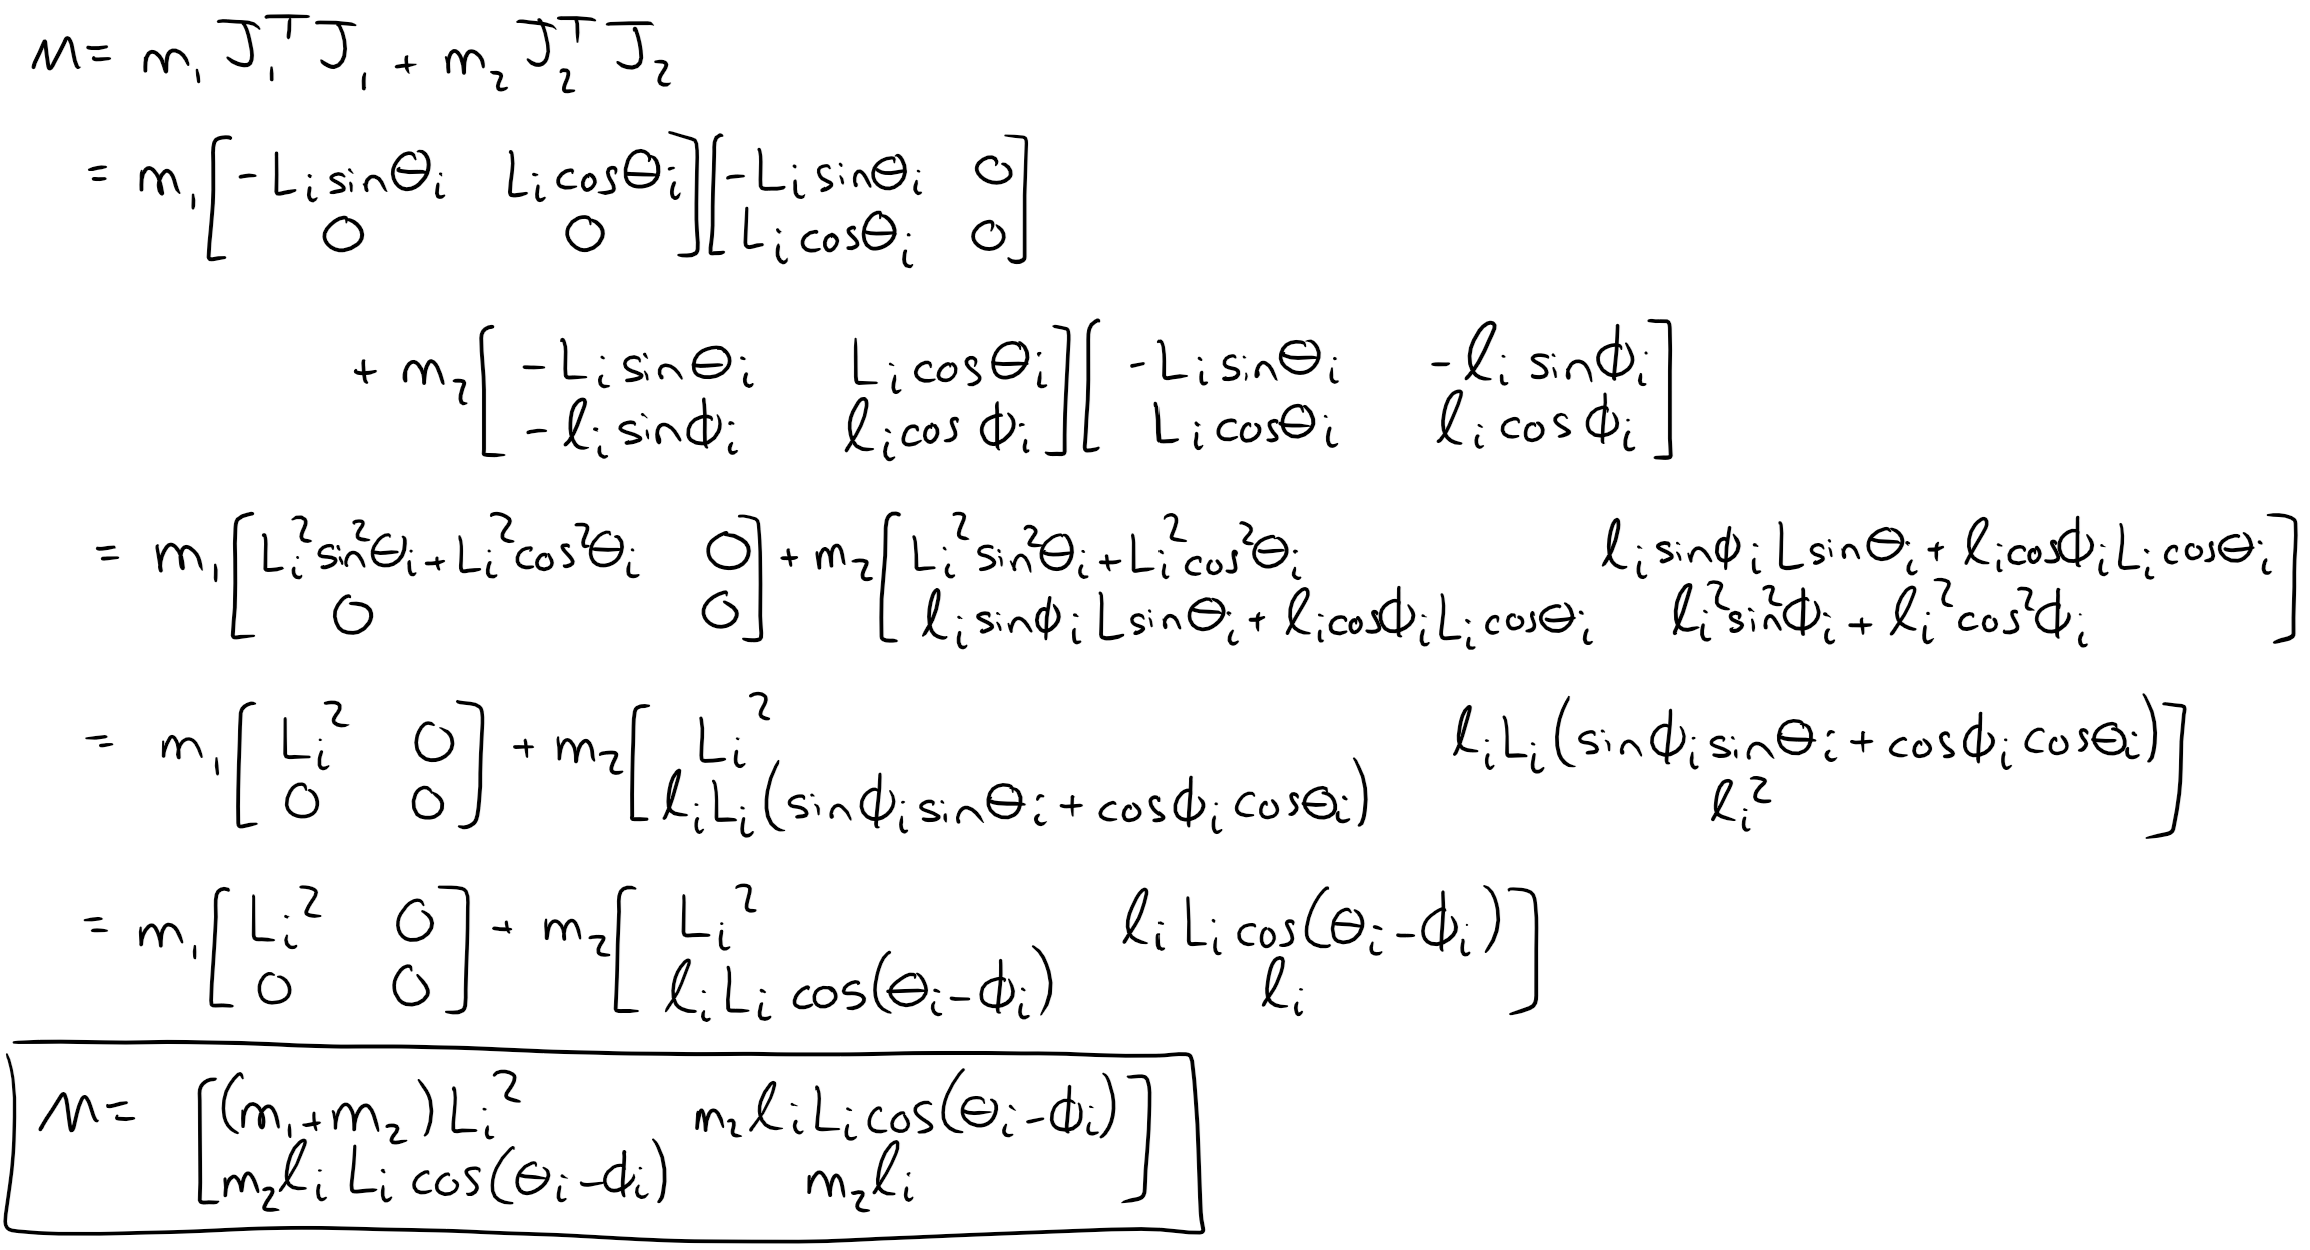
\includegraphics[width=\textwidth]{7_Appendices/img/too_much_math_to_write.png}
    \caption{Simplification Steps for Inertia Matrix}
    \label{fig:inertia_matrix_simplification}
\end{figure}

The generalized equation of motion takes the form

\begin{equation} \label{eq:dynamic_general}
    M\Ddot{\theta} + c(\theta,\dot{\theta}) + \mu (\dot{\theta}^2) + G(\theta) + F(\theta) = \tau
\end{equation}

where $c(\theta,\dot{\theta})$ is the coriolis effect, $\mu (\dot{\theta}^2)$ is the centrifugal effect, $G(\theta)$ is gravity, $F(\theta)$ is the force applied at the foot and $\tau$ is the joint torques.
Coriolis and centrifugal forces have been neglected to simplify analysis.
$G(\theta)$ is given by

\begin{equation} \label{eq:gravity_matrix}
    G(\theta) = g \begin{bmatrix}
        (m_1 + m_2) L \cos\theta + m_2 \ell \cos\theta \\
        m_2 \ell \cos\phi
    \end{bmatrix}
    = [m/s^2]([kg][m]) = [Nm]
\end{equation}

where $g = 9.81 m/s^2$.
The force matrix $F(\theta)$ is

\begin{equation} \label{eq:force_matrix}
    F(\theta) = N \begin{bmatrix}
        L\cos\theta + \ell\cos\phi \\
        \ell\cos\phi
    \end{bmatrix} + f \begin{bmatrix}
        L\sin\theta + \ell\sin\phi \\
        \ell\sin\phi
    \end{bmatrix}
    = [N][m]
\end{equation}

where $N$ is the normal force at the foot and $f$ is the friction force at the foot.
Friction force in the $y$ plane was neglected as it should not directly impact the joint torques, except through increasing the friction in bearings, etc.
Finally, equations \ref{eq:gravity_matrix} and \ref{eq:force_matrix} are inserted into \ref{eq:dynamic_general} giving the final generalized equation of motion

\begin{equation} \label{eq:dynamic_equation_app}
    \begin{split}
        \begin{bmatrix} 
            (m_1 + m_2) L^2 & m_2 \ell L \cos(\theta-\phi) \\
            m_2 \ell L \cos(\theta-\phi) & m_2 \ell
        \end{bmatrix}
        \begin{bmatrix} \Ddot{\theta} \\ \Ddot{\phi} \end{bmatrix}
        +
        g \begin{bmatrix}
            (m_1 + m_2) L \cos\theta + m_2 \ell \cos\theta \\
            m_2 \ell \cos\phi
        \end{bmatrix} \\
        +
        N \begin{bmatrix}
            L\cos\theta + \ell\cos\phi \\
            \ell\cos\phi
            \end{bmatrix} + f \begin{bmatrix}
            L\sin\theta + \ell\sin\phi \\
            \ell\sin\phi
        \end{bmatrix}
        =
        \begin{bmatrix}
        \tau_1 \\ \tau_2
        \end{bmatrix}
    \end{split}
\end{equation}

where $\tau_1$ and $\tau_2$ are the joint torques for the hip and knee, respectively.

%------------------------- Force at feet -------------------------%

\subsection{Force at Feet}
\label{app:feet_force}
These equations were first tried to calculate the force at every feet of the robot, however after calculation it was determined to be a statically indeterminate system. 

\begin{gather}
    \sum F_z = 0 = N_A + N_B +N_C + N_D +N_E -mg
    \\
    \sum M_{x_A} = 0 = -N_E r_{EA_y} + N_D r_{DA_y} + N_B r_{BA_y} + N_C r_{CA_y} - mg r_{gA_y}
    \\
    \sum M_{x_E} = 0 = N_A r_{AE_y} N_D r_{DE_y} + N_B r_{BE_y} + N_C r_{CE_y} - mg r_{gE_y}
    \\
    \sum M_{y_A} = 0 = N_E r_{EA_x} + N_D r_{DA_x} + N_C r_{CA_x} -mg r_{gA_x}
    \\
    \sum M_{y_B} = 0 = N_E r_{EB_x} + N_D r_{DB_x} + N_C r_{CB_x} -mg r_{gB_x}
\end{gather}

What if there is force in different directions (Complete 3D), must look at matrices?

\begin{gather}
    M_j = \sum (r_i \times N_i) + mg
    \\
    M_{j_x} = \sum(r_{i_y} N_{i_z} - r_{i_z} N_{i_y}) + ...
    \\
    M_{j_y} = \sum(r_{i_z} N_{i_x} - r_{i_x} N_{i_z}) +...
    \\
    M_{j_z} = \sum(r_{i_x} N_{i_y} - r_{i_y} N_{i_x}) + ...
\end{gather}

%------------------------- DRAG FORCES -------------------------%
\subsection{Drag Coefficients} \label{app:drag_coeff}

The drag coefficient acting on the robot was obtained with Figure \ref{fig:drag_coef}. The most appropriate shape is the rectangle with the values $D = h = 200 mm$, $l = d = 600 mm$, and $ b = w = 1000 mm$. Therefore, we obtain a ratio of $l/D = d/h = 600 mm / 200 mm = 3$ and based on the table from Figure \ref{fig:drag_coef}, $C_{D} = 1.3$. Finally, the reference area $A = bD = wh = (1 m)(0.2 m) = 0.2 m^2$.

\begin{figure}[H]
    \centering
    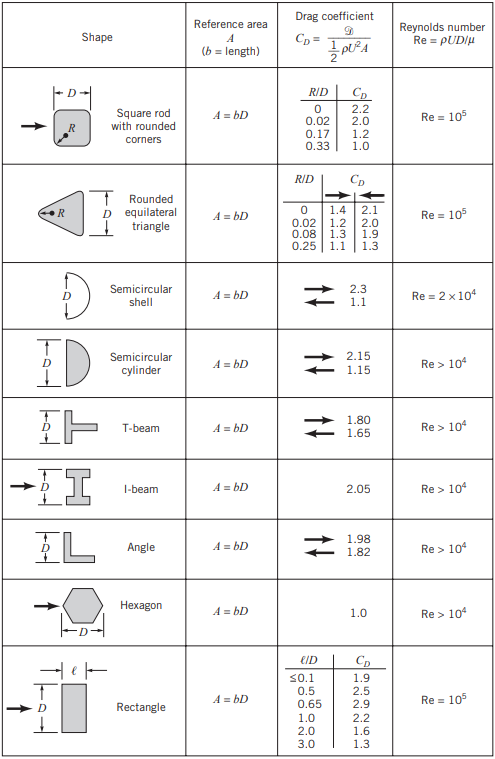
\includegraphics{7_Appendices/img/drag_coefficients.PNG}
    \caption{Various Drag Coefficients for Two-Dimensional Objects \cite{munson_fundamentals_2009}} 
    \label{fig:drag_coef}
\end{figure}

%------------- BATTERY CODE - RUNTIME IN, DIMENSIONS OUT -------------%
\subsection{Battery Sample Code} \label{app:battery}
\noindent\begin{minipage}{\textwidth}
    \begin{lstlisting}[language=Matlab,caption=Battery dimension calculator - Basic]
    function [x,y,z] = getBatteryDimensionsSingle(number_of_cells,number_of_batteries): 
        
        % Battery dimensions in mm and g
        D = 18.24;
        H = 65.1;
        
        [cells_per_battery,remainder] = quorem(number_of_cells,number_of_batteries)
        if(remainder != 0):
            cells_per_battery = cells_per_battery + 1;
        end
        
        % cells are arranged upright, 1 high, with even width and length if possible
        cells_wide_square = sqrt(cells_per_battery);
        cells_wide = floor(cells_wide_square);
        cells_long = ceil(cells_wide_square);
        
        x = cells_wide * D;
        y = cells_long * D;
        z = H;
    \end{lstlisting}
\end{minipage}

The chassis dimensions could then be found programmatically by multiplying the battery dimensions by some constant (for example, $h_{chassis} = 1.5 h_{battery}$, then ensuring that this length is also sufficient to allow the desired range of motion of the leg

\subsection{Centre of Mass Calculation} \label{app:centre_of_mass}

\begin{table}[H]
\centering
  \caption{Centre of Mass Calculation and Components' Location}
  \label{table:weight_distribution}
  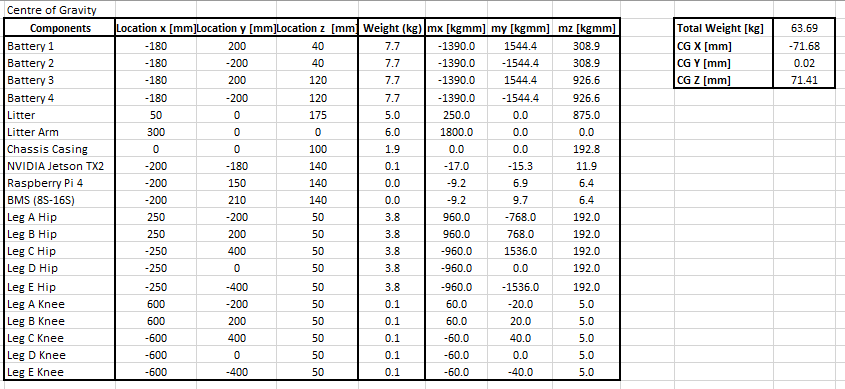
\includegraphics[width=\textwidth]{7_Appendices/img/WeightDistribution.PNG}
\end{table}

%------------------------- DATA SHEETS -------------------------%
\section{Data Sheets} \label{app:data_sheets}

%\begin{comment}
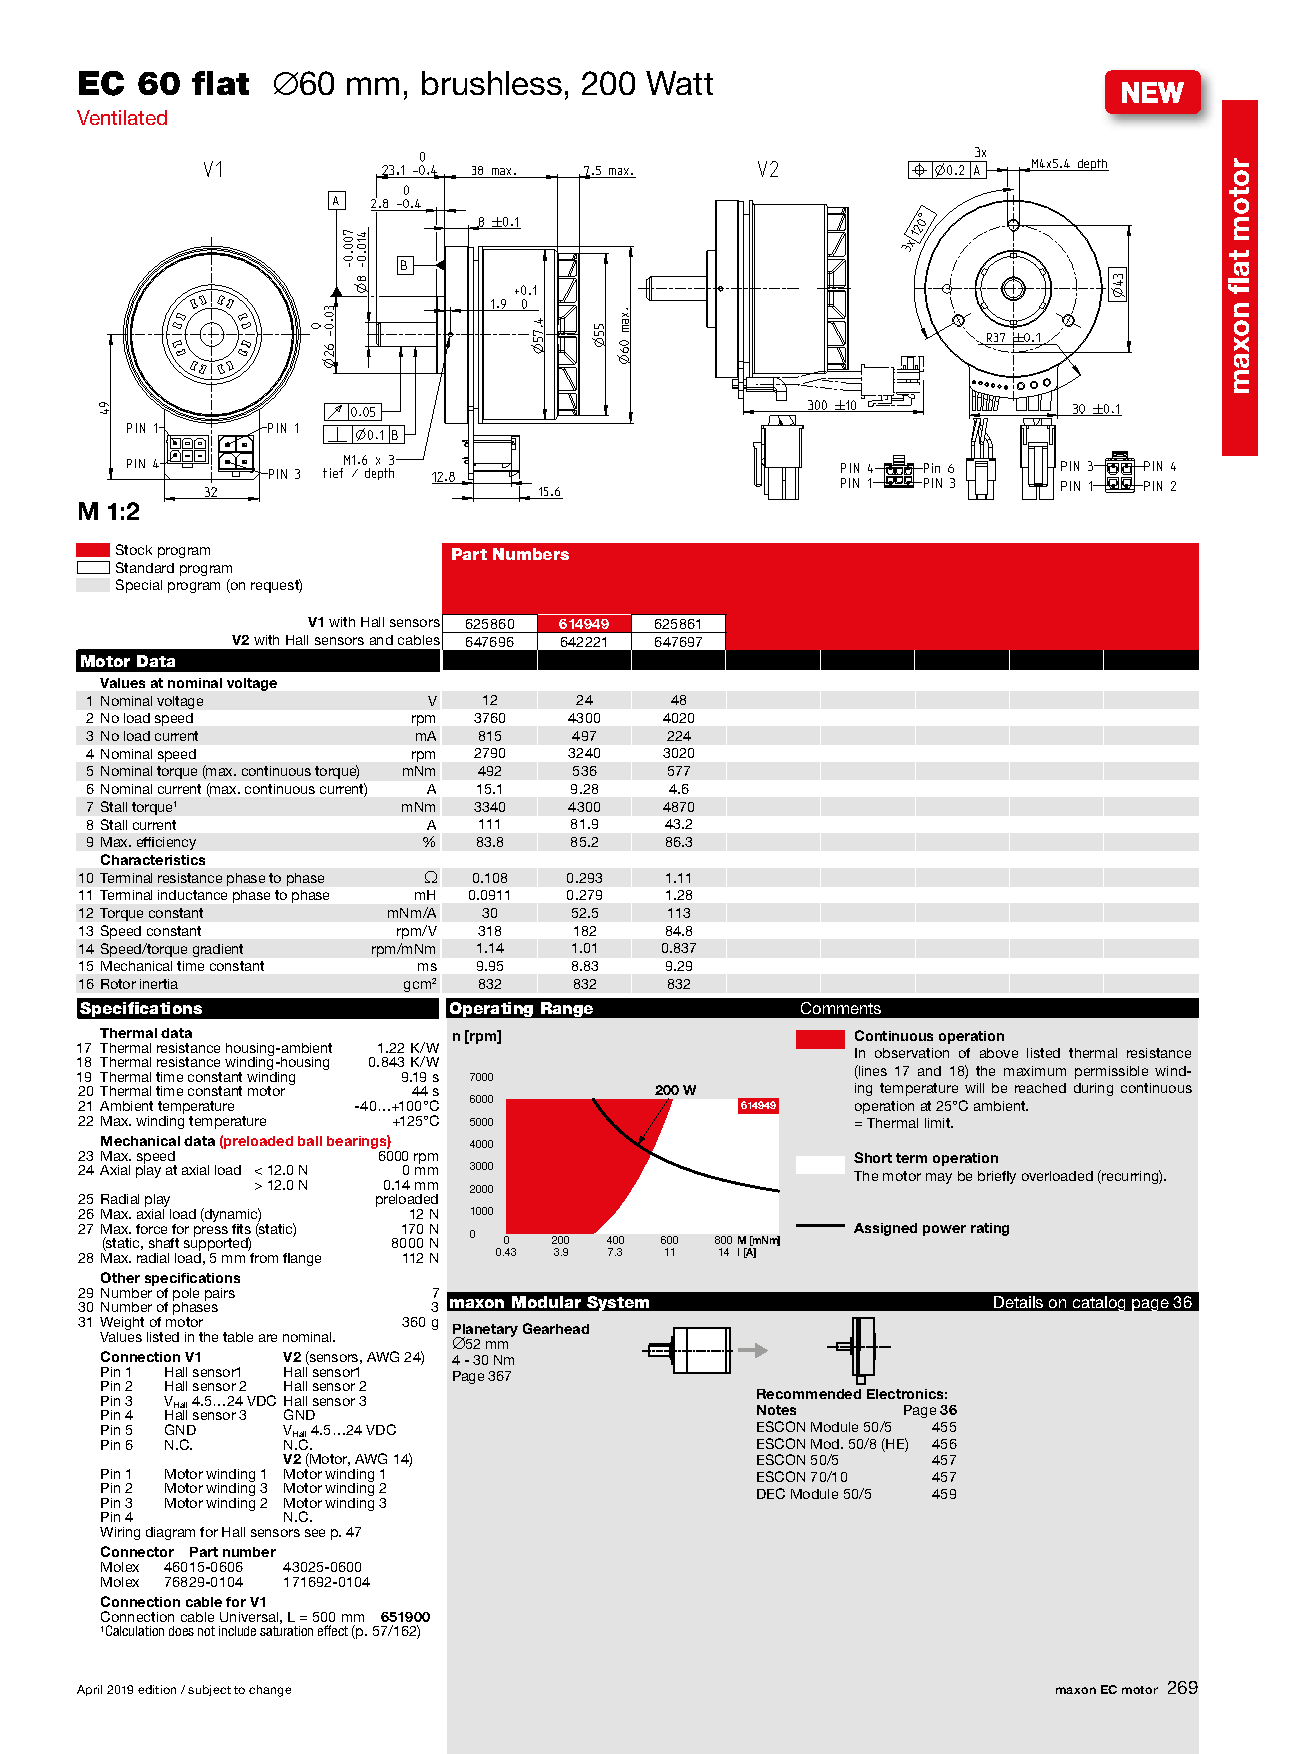
\includepdf[pages=-]{pdf/maxon_ec60_200w.pdf}
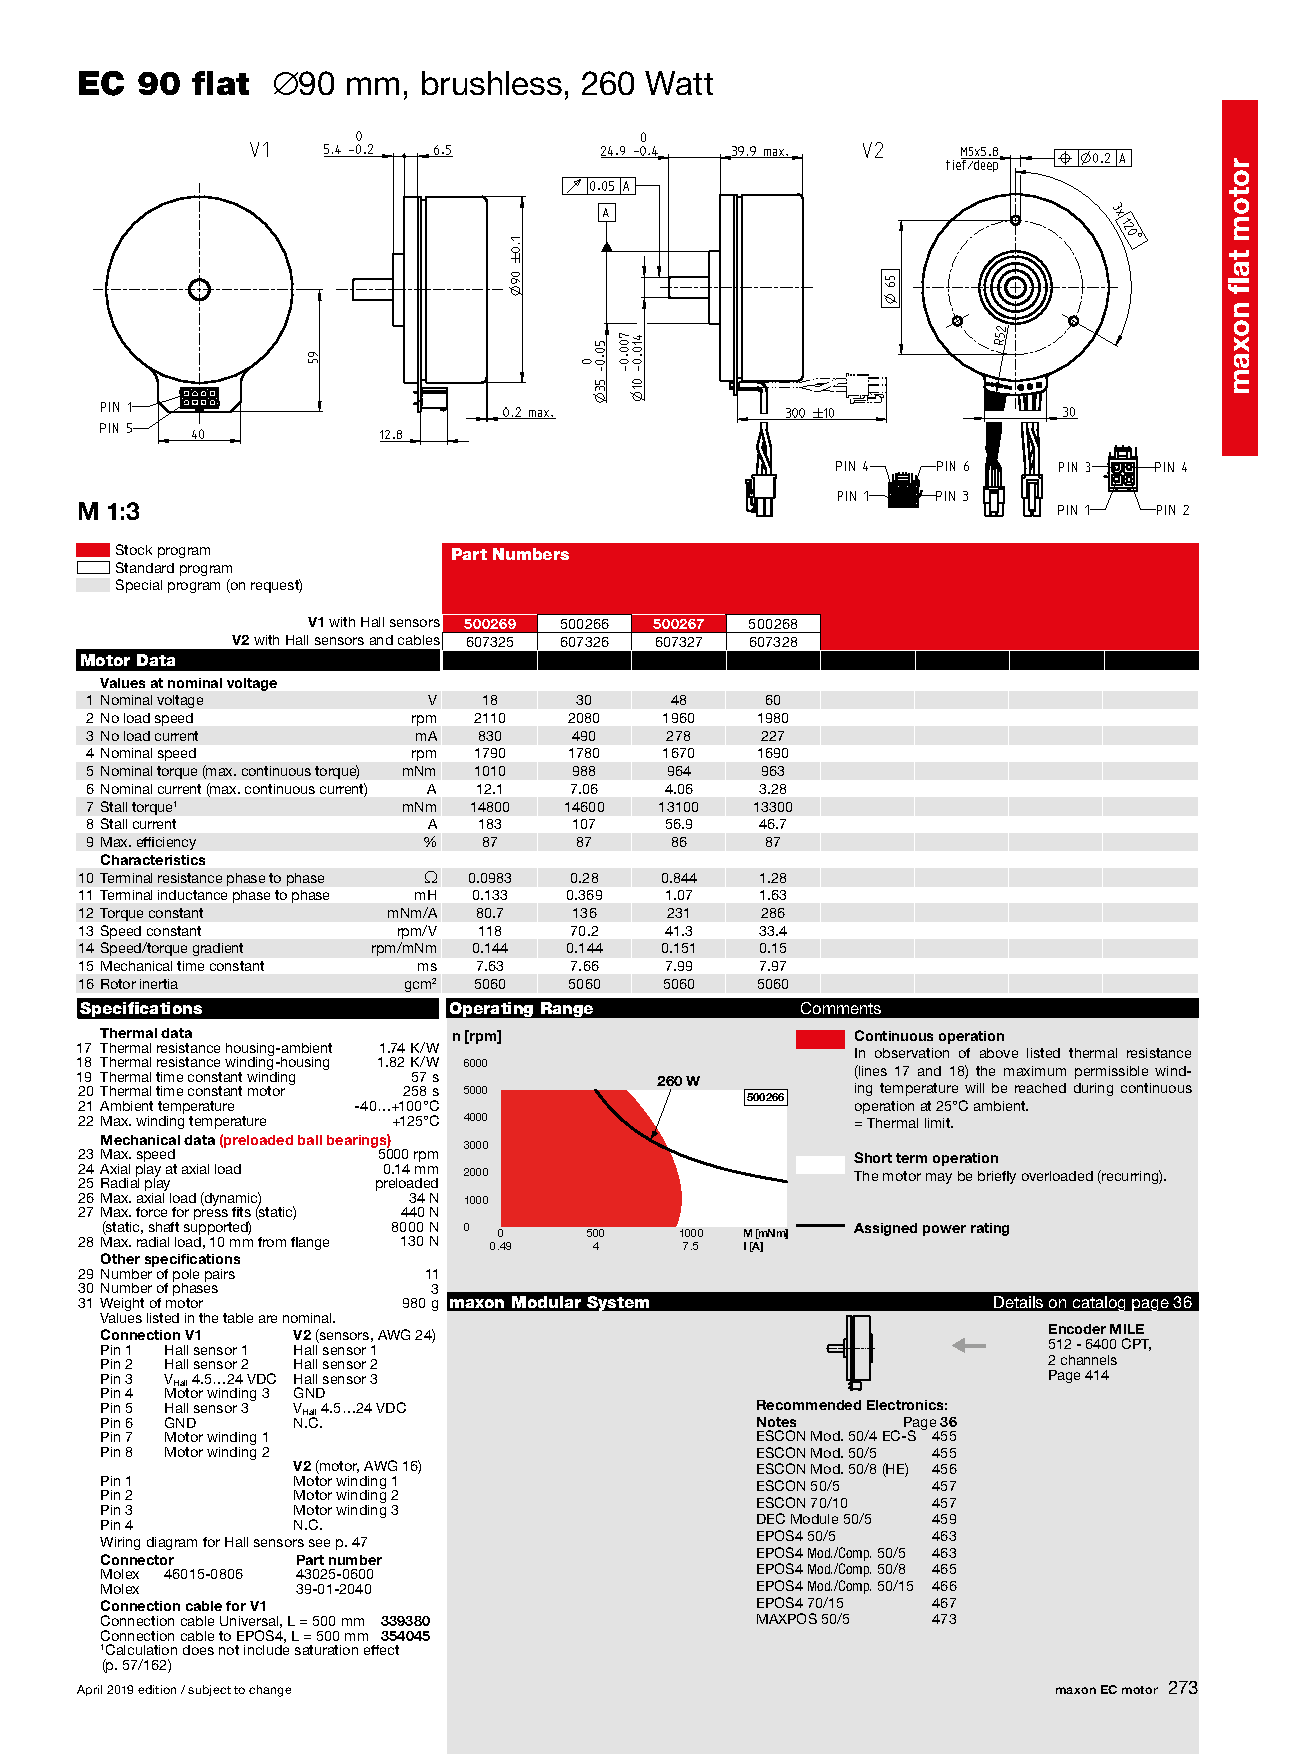
\includepdf[pages=-]{pdf/maxon_ec90_260w.pdf}
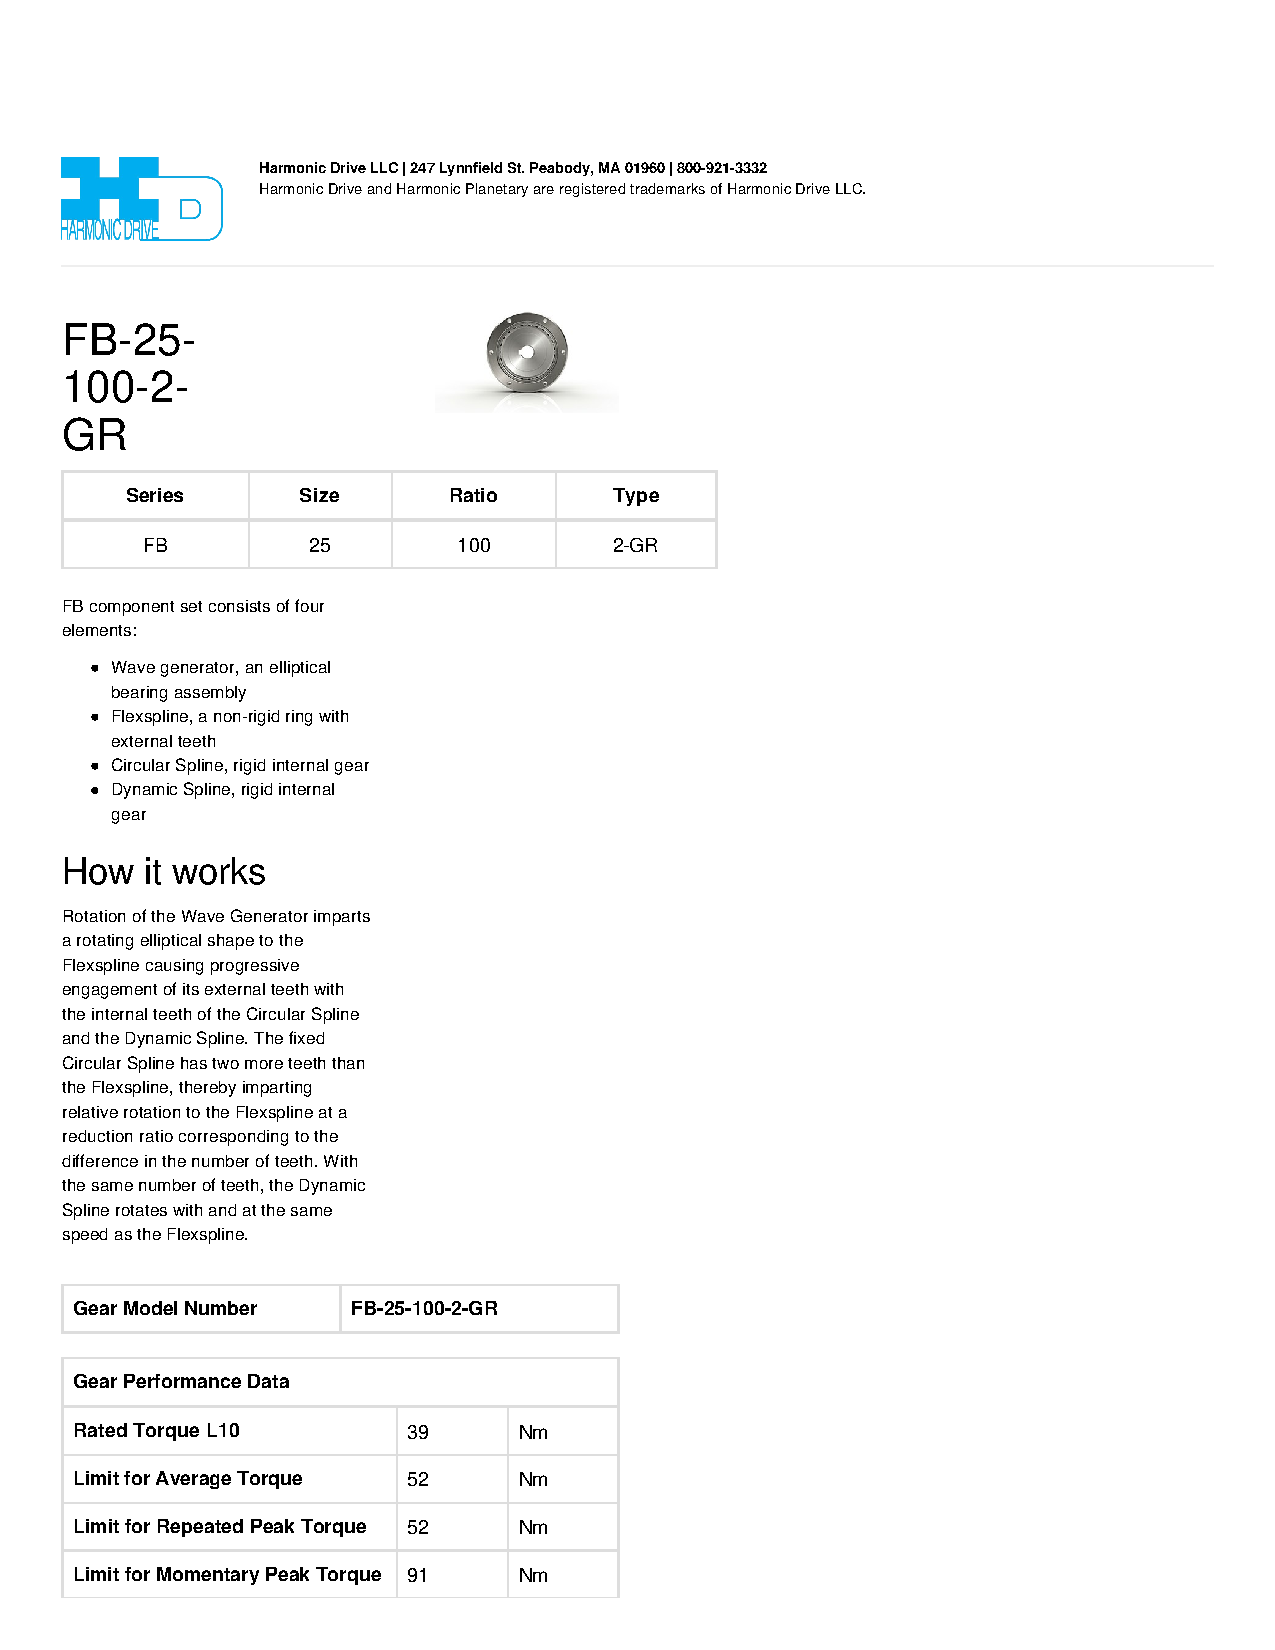
\includepdf[pages=-]{pdf/FB-25-100-2-GR.pdf}
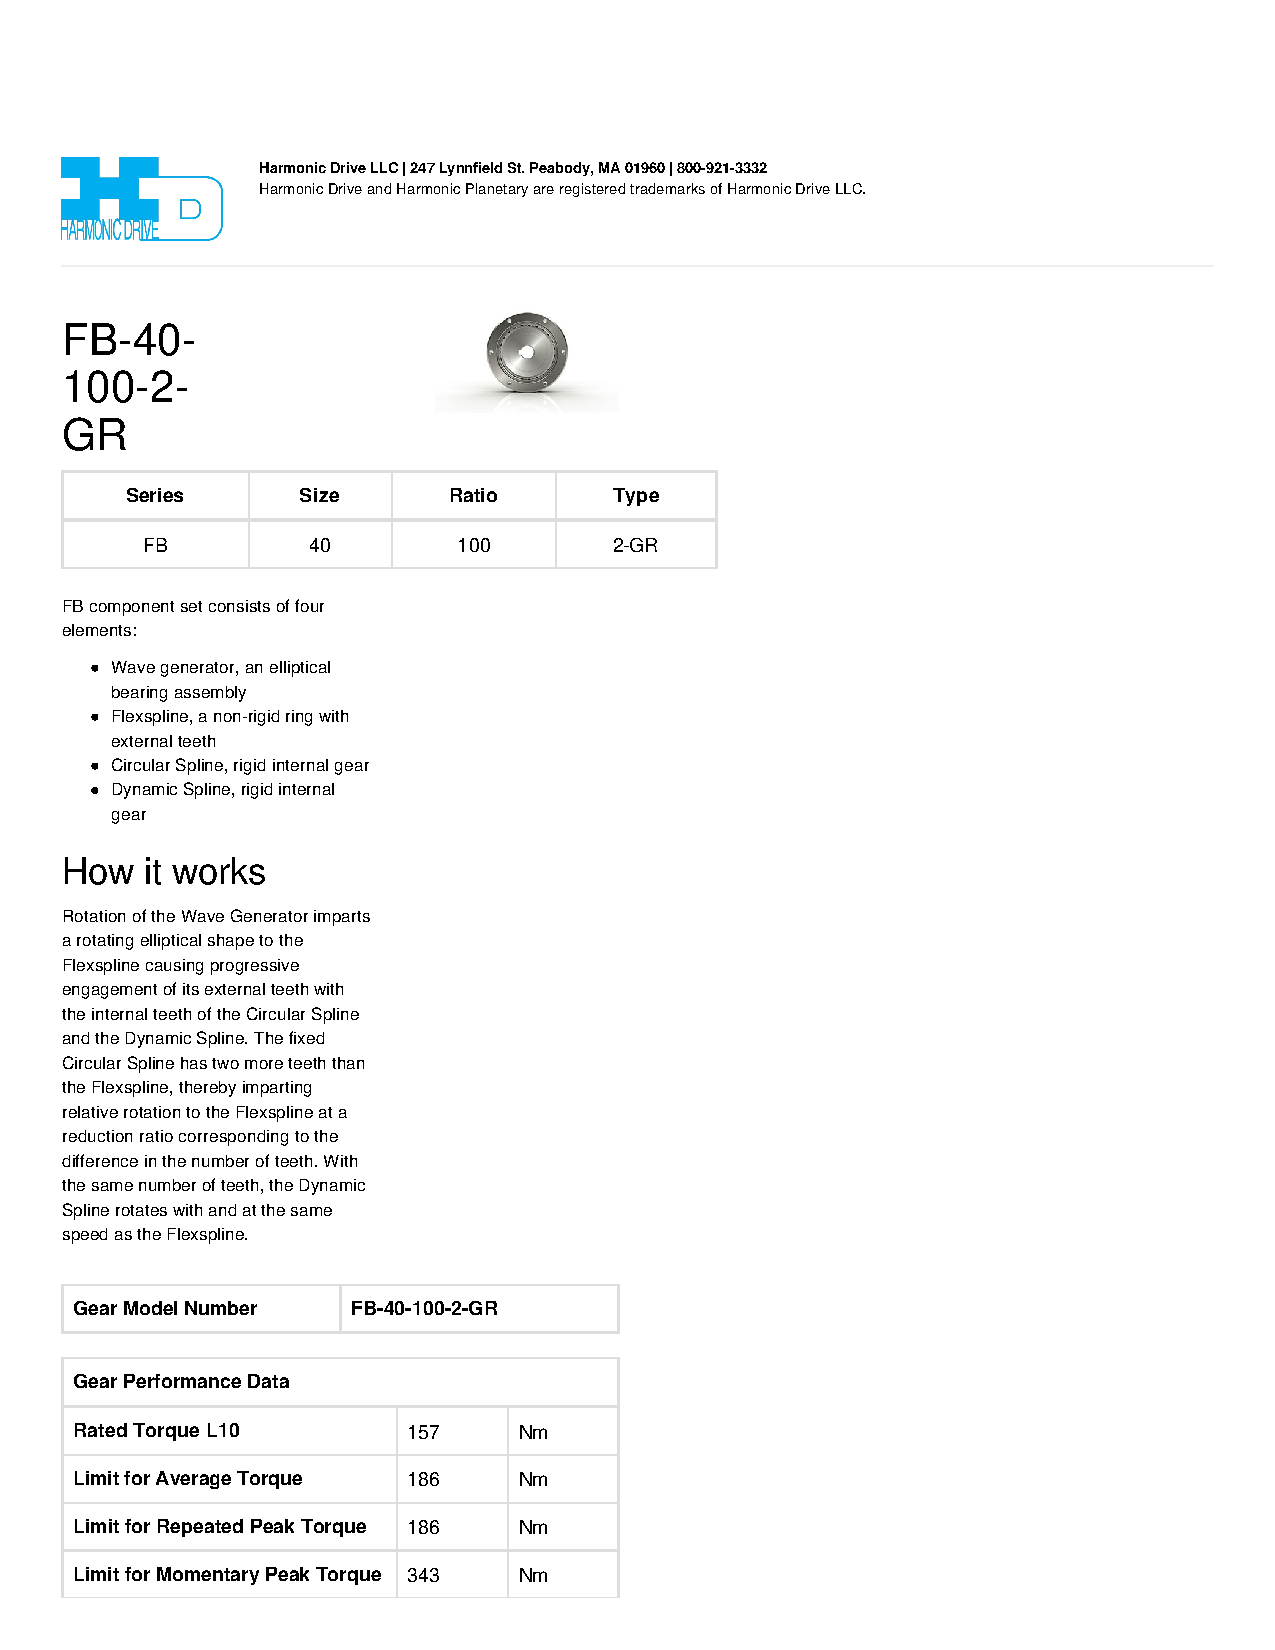
\includepdf[pages=-]{pdf/FB-40-100-2-GR.pdf}
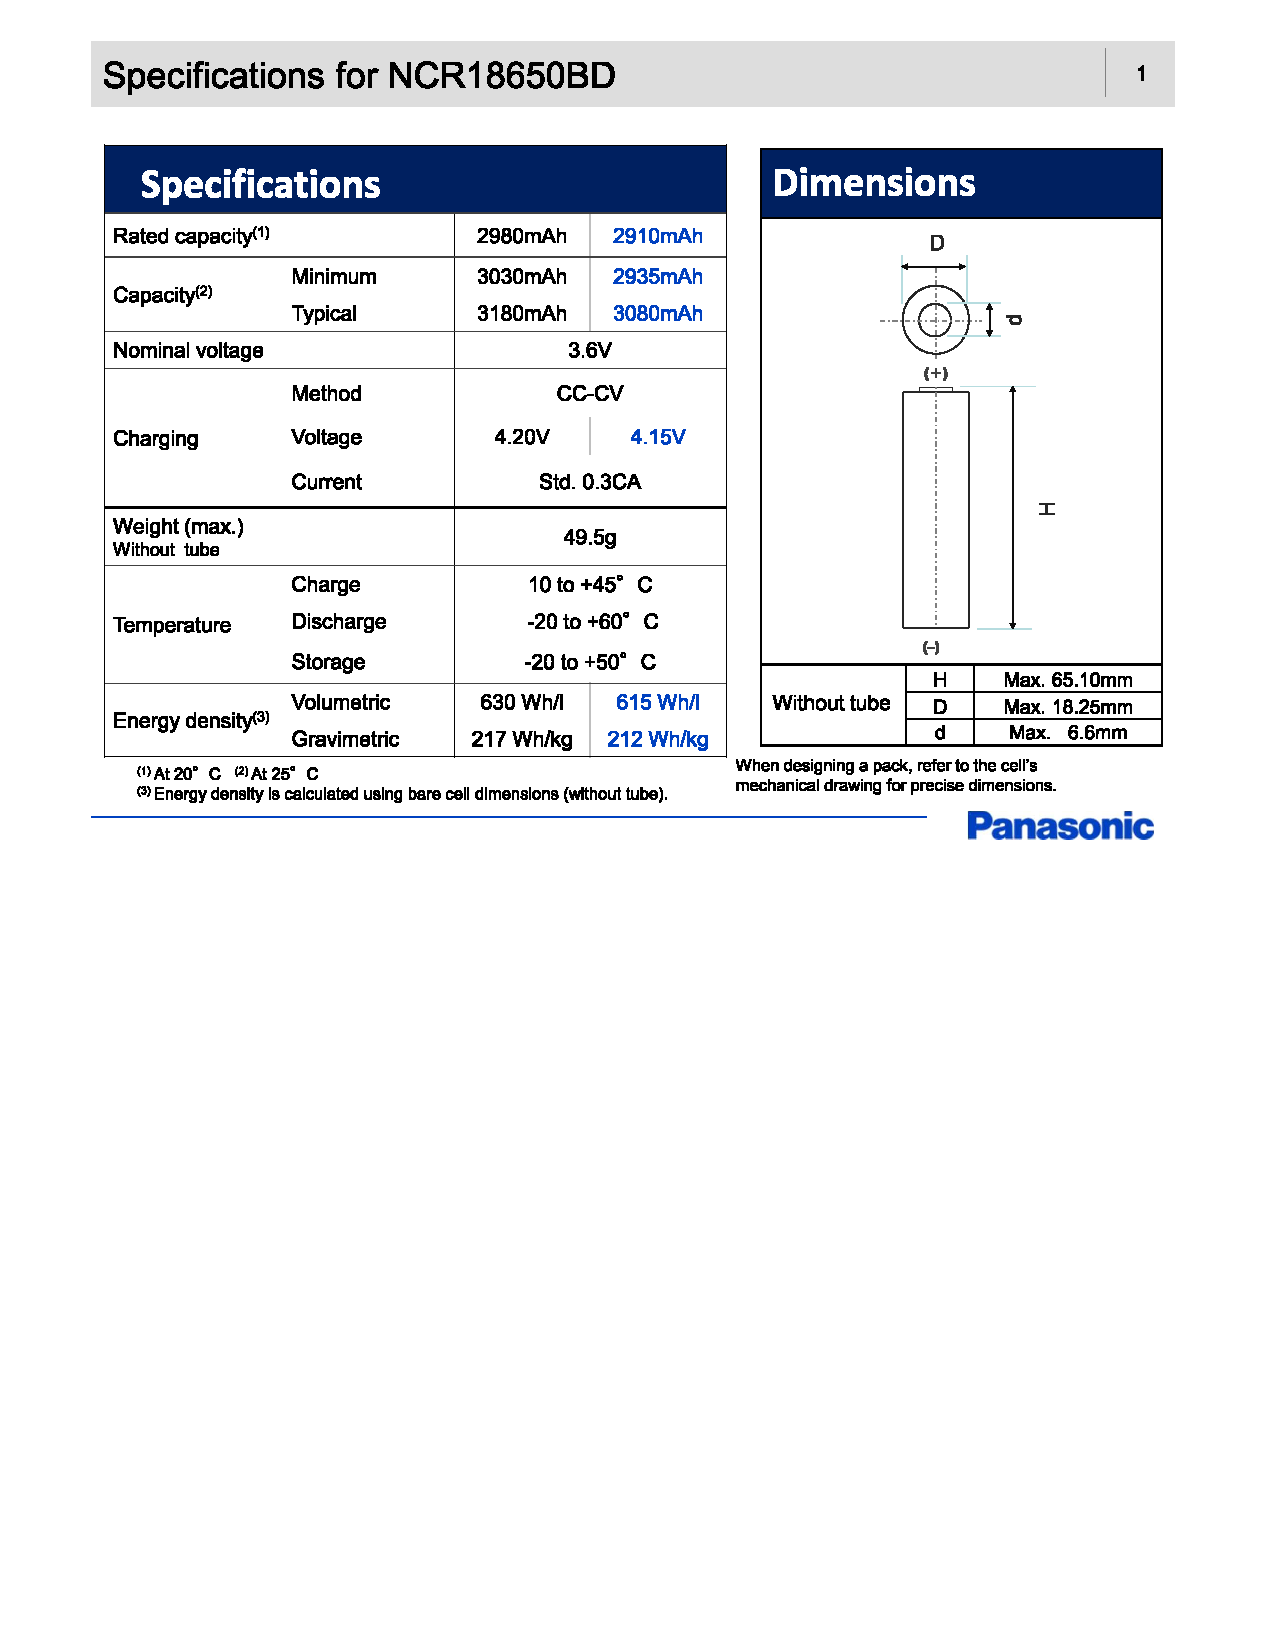
\includepdf[pages=-]{pdf/panasonic_18650.pdf}
%\end{comment}